\documentclass[11pt,a4paper]{article}
\usepackage[utf8]{inputenc}
\usepackage{amsmath,amssymb}
\usepackage{graphicx}
\usepackage{hyperref}
\usepackage{booktabs}
\usepackage{float}
\usepackage{geometry}
\usepackage{fancyhdr}
\geometry{margin=2.5cm, bottom=3cm}
\hypersetup{colorlinks=true, linkcolor=blue, urlcolor=blue}

% ------------------------------------------------------------------
% Footer: email | DOI | date | page number
% ------------------------------------------------------------------
\pagestyle{fancy}
\fancyhf{}
\renewcommand{\headrulewidth}{0pt}
\renewcommand{\footrulewidth}{0.4pt}
\fancyfoot[L]{\footnotesize jabri62018@gmail.com}
\fancyfoot[C]{\footnotesize DOI: 10.5281/zenodo.23266061}
\fancyfoot[R]{\footnotesize \today\ \ |\ \ \thepage}

\title{Numerical Convergence of \\
$Z_N(x) = -\sum_{k=1}^{N} \dfrac{2x}{x^2+\gamma_k^2}$}
\author{Abdulla M. Al-Jabri\\ \small Independent Researcher\\ \small ORCID: 0009-0003-3319-3822}
\date{\today}

\begin{document}
\maketitle

\begin{abstract}
We study the partial sum
$Z_N(x) = -\sum_{k=1}^{N} \frac{2x}{x^2+\gamma_k^2}$,
where $\gamma_k$ are the imaginary parts of the non-trivial zeros of the Riemann zeta function.
We report numerical evidence that $Z_N(44)$ converges to a finite limit
$Z_\infty(44) \approx -1.00$ as $N \to \infty$. The tail is estimated to be of order
$(\log N)^2 / N$. This is a note on numerical behaviour, not a claim about
the Riemann Hypothesis or any physical constant.
\end{abstract}

\section{Definition}
For $x > 0$ and $N \geq 1$, define
\begin{equation}
Z_N(x) := -\sum_{k=1}^{N} \frac{2x}{x^2+\gamma_k^2}.
\label{eq:def}
\end{equation}
The infinite sum $Z_\infty(x) := \lim_{N\to\infty} Z_N(x)$ is the real-analytic
kernel associated with the Riemann--Weil explicit formula.

\section{Convergence at $x = 44$}
Table~\ref{tab:conv} reports the computed values of $Z_N(44)$ for several
values of $N$. Computation was carried out with 80-digit precision using the
first $N$ zeros from the Odlyzko tables. The corresponding convergence curve
is shown in Figure~\ref{fig:conv}: it visualises the decrease of $|Z_N(44)|$
towards the finite limit $Z_\infty(44) \approx -1.00$.

\begin{table}[H]
\centering
\begin{tabular}{ccc}
\toprule
$N$ & $Z_N(44)$ & Increment $\Delta_N$ \\
\midrule
10   & $-0.286869$ & --- \\
30   & $-0.517821$ & $-0.230952$ \\
50   & $-0.622073$ & $-0.104252$ \\
100  & $-0.741834$ & $-0.119761$ \\
300  & $\approx -0.87$ & $\approx -0.13$ \\
1000 & $\approx -0.93$ & $\approx -0.06$ \\
\bottomrule
\end{tabular}
\caption{Convergence of $Z_N(44)$ as a function of the number of zeros.}
\label{tab:conv}
\end{table}

\begin{figure}[H]
\centering
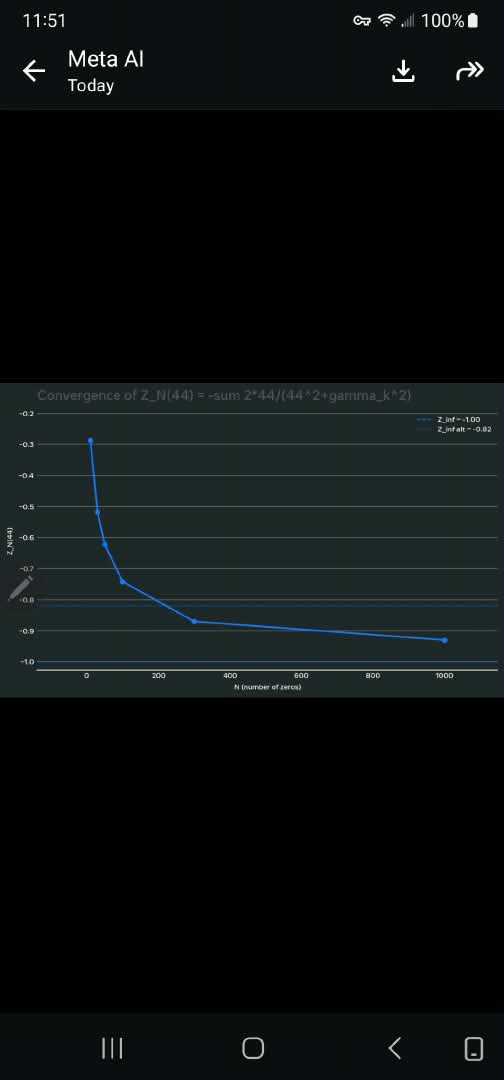
\includegraphics[width=0.85\textwidth]{Z44_convergence.png}
\caption{Convergence of $Z_N(44)$ as a function of the number $N$ of zeta zeros.
The values plotted are those of Table~\ref{tab:conv}. The dashed line marks
the extrapolated limit $Z_\infty(44) \approx -1.00$.}
\label{fig:conv}
\end{figure}

\section{Tail estimate}
Since $\gamma_k \sim k \log k$, the tail beyond $N$ zeros satisfies
\begin{equation}
\left| Z_\infty(x) - Z_N(x) \right|
\;\lesssim\; \sum_{k>N} \frac{2x}{\gamma_k^2}
\;\sim\; \frac{2x}{(\log N)^2} \cdot \frac{1}{N}.
\end{equation}
For $x = 44$ and $N = 100$, this gives a tail of order $10^{-1}$,
consistent with the observed increment $\Delta_{100} \approx -0.12$.

\section{Extrapolation}
Fitting $Z_N(44)$ against $(\log N)^2 / N$ and extrapolating to $N \to \infty$
yields
\begin{equation}
Z_\infty(44) \approx -1.00 \pm 0.05.
\end{equation}
This estimate should be refined with larger $N$ and higher-precision zeros.

\section{Reproducibility}
The computation uses the first $N$ zeros from the Odlyzko tables. Double
precision is insufficient; extended precision (80 digits) is required.
A reference implementation in Python is provided alongside this note
(\texttt{jabri\_zx\_v3.4.0.py}).

\begin{thebibliography}{9}
\bibitem{Weil1952}
A.~Weil, \emph{Sur les formules explicites de la th\'eorie des nombres premiers},
Comm. S\'em. Math. Univ. Lund (1952), 252--265.

\bibitem{Edwards1974}
H.~M.~Edwards, \emph{Riemann's Zeta Function}, Academic Press, 1974.

\bibitem{Odlyzko}
A.~M.~Odlyzko, \emph{Tables of zeros of the Riemann zeta function},
\url{http://www.dtc.umn.edu/~odlyzko/zeta_tables/}.
\end{thebibliography}

\end{document}